\documentclass[12pt,a4paper,oneside]{report}
\usepackage{src/styles/report_style}

\begin{document}
\hypersetup{pageanchor=false}

% --- BAGIAN AWAL ---
\pagenumbering{roman}

\begin{titlepage}
	\thispagestyle{empty}
	\centering
	% \vspace*{1.5cm}

	{\large \bfseries LAPORAN AKHIR MAGANG MANDIRI\par}
	\vspace{1cm}

	{\large \bfseries FRONTEND DEVELOPER\par}
	{\large \bfseries PT VORTEX BUANA EDUMEDIA\par}
	\vspace{2cm}

	
\includegraphics[width=5cm]{assets/images/logo-ugm.png}
	\par\vspace{2cm}

	{\large \bfseries Disusun oleh:\par}
	{\large \bfseries Andreandhiki Riyanta Putra\par}
	{\large \bfseries 23/517511/PA/22191\par}
	\vspace{3cm}

	{\large \bfseries PROGRAM STUDI S1 ILMU KOMPUTER\par}
	{\large \bfseries DEPARTEMEN ILMU KOMPUTER DAN ELEKTRONIKA\par}
	{\large \bfseries FAKULTAS MATEMATIKA DAN ILMU\par}
	{\large \bfseries PENGETAHUAN ALAM\par}
	{\large \bfseries UNIVERSITAS GADJAH MADA\par}
	{\large \bfseries YOGYAKARTA\par}
	{\large \bfseries 2026\par}

\end{titlepage}

\setcounter{page}{2}
% \chapter*{Lembar Pengesahan}
\addcontentsline{toc}{chapter}{Lembar Pengesahan}

\noindent Laporan kegiatan Magang MBKM ini disusun oleh:
\vspace{0.5cm}

\begin{tabular}{ll}
Nama & : Andreandhiki Riyanta Putra \\
NIM & : 23/XXXXXX/PA/XXXXX \\
Program Studi & : Ilmu Komputer \\
Tempat Magang & : Facetology (Jakarta Selatan) \\
\end{tabular}

\vspace{1cm}
\noindent Telah diperiksa dan disetujui pada tanggal: ................................

\vspace{2cm}
\begin{center}
\small
\begin{tabular}{@{}>{\centering\arraybackslash}p{0.40\textwidth}p{0.06\textwidth}>{\centering\arraybackslash}p{0.40\textwidth}@{}}
    Dosen Pembimbing Akademik & & Pembimbing Lapangan / Mentor \\
    & & \\
    & & \\
    & & \\
    \underline{(Nama Dosen Pembimbing)} & & \underline{(Nama Mentor)} \\
    NIP. XXXXXXXXXXXXXXXX & & NIK. XXXXXXXXX \\
\end{tabular}
\normalsize
\end{center}
% \chapter*{Kata Pengantar}
\addcontentsline{toc}{chapter}{Kata Pengantar}

Puji syukur penulis panjatkan kehadirat Tuhan Yang Maha Esa atas segala rahmat dan karunia-Nya sehingga penulis dapat menyelesaikan Laporan Akhir Magang MBKM ini dengan baik. Laporan ini disusun sebagai bentuk pertanggungjawaban dan dokumentasi atas kegiatan Magang Mandiri yang dilaksanakan di PT Vortex Buana Edumedia, Yogyakarta.

Penulis menyampaikan terima kasih kepada pihak-pihak yang telah mendukung pelaksanaan magang dan penyusunan laporan ini. Terima kasih kepada Dosen Pembimbing Akademik yang telah memberikan arahan akademik selama kegiatan magang berlangsung. Terima kasih kepada pembimbing lapangan dan rekan tim di PT Vortex Buana Edumedia yang telah membimbing, berbagi pengetahuan, dan memberikan kesempatan untuk berkontribusi pada proyek-proyek internal perusahaan. Terima kasih pula kepada Program Studi Ilmu Komputer dan Departemen Ilmu Komputer dan Elektronika, Fakultas Matematika dan Ilmu Pengetahuan Alam, Universitas Gadjah Mada, yang telah menyelenggarakan program MBKM sehingga mahasiswa dapat memperoleh pengalaman kerja langsung di lingkungan industri.

Penulis menyadari bahwa laporan ini masih dapat diperbaiki. Kritik dan saran yang membangun sangat penulis harapkan demi penyempurnaan laporan ini di kemudian hari.

\vspace{1.5cm}
\begin{flushright}
Yogyakarta, Februari 2026\\[1.5cm]
Penulis
\end{flushright}

% Daftar Isi, Gambar, Tabel
\clearpage
\phantomsection
\addcontentsline{toc}{chapter}{Daftar Isi}
\tableofcontents
\clearpage
\phantomsection
\addcontentsline{toc}{chapter}{Daftar Gambar}
\listoffigures
\clearpage
\phantomsection
\addcontentsline{toc}{chapter}{Daftar Tabel}
\listoftables
\clearpage

% --- BAGIAN UTAMA ---
\hypersetup{pageanchor=true}
\pagenumbering{arabic}

\chapter{Profil Perusahaan dan Kegiatan MBKM}

\section{Profil Perusahaan}
PT Vortex Buana Edumedia merupakan perusahaan teknologi dan transformasi digital yang berpusat di Yogyakarta. Vortex berfokus pada pengembangan solusi perangkat lunak end-to-end untuk kebutuhan pendidikan dan bisnis, baik melalui produk internal maupun layanan pengembangan digital. Dalam ekosistem produknya, Vortex mengembangkan Neon, yang mencakup Neon Uji dan Neon Belajar. Neon Uji menyediakan kuis on-demand, tryout, laporan hasil yang rinci, serta fitur pemantauan progres peserta yang mendukung proses evaluasi pembelajaran secara lebih terstruktur. Selain pengembangan produk, Vortex juga menyediakan layanan pengembangan web dan media digital yang mendukung kebutuhan transformasi digital mitra dan pengguna.

\section{Penjelasan Program Magang}
Selama program MBKM Independen, saya melaksanakan magang selama tiga bulan, terhitung sejak 3 November 2025 hingga 3 Februari 2026, sebagai Frontend Developer pada divisi Product di PT Vortex Buana Edumedia. Pada kegiatan ini, saya terlibat dalam pengembangan beberapa produk internal yang berfokus pada penguatan ekosistem Neon serta penyempurnaan pengalaman pengguna pada sistem yang sedang berjalan.

Proyek pertama yang saya kerjakan adalah Neutron Office, yaitu sistem integrasi yang menghubungkan rekam belajar dengan nilai dari Neon Uji. Sistem ini dirancang untuk menyatukan data pembelajaran dan penilaian agar dapat dikelola secara lebih rapi dan mudah diakses. Kontribusi saya pada proyek ini berfokus pada pengembangan antarmuka frontend, penyesuaian alur interaksi pengguna, serta implementasi komponen yang mendukung integrasi data dengan tampilan yang jelas dan mudah digunakan.

Proyek kedua adalah Neon Uji SaaS, yaitu platform asesmen yang digunakan untuk kebutuhan kuis, tryout, dan evaluasi pembelajaran. Pada proyek ini, saya berperan dalam perbaikan bug, peningkatan kualitas antarmuka, serta penyempurnaan pengalaman pengguna agar sistem lebih stabil, konsisten, dan nyaman digunakan pada berbagai skenario penggunaan. Pengerjaan ini menuntut ketelitian tinggi karena perubahan kecil pada antarmuka dapat memengaruhi alur penggunaan secara keseluruhan.

Proyek ketiga adalah Neon Interfaces, yaitu dokumentasi design library yang berfungsi sebagai referensi komponen antarmuka bagi tim desain dan pengembangan. Pada proyek ini saya membantu menyusun dokumentasi komponen, membangun basis design library yang mengacu pada shadcn/ui, serta menjaga konsistensi pola UI agar dapat digunakan kembali pada proyek-proyek internal lain. Pengembangan ini mendukung standarisasi tampilan sekaligus mempercepat implementasi antarmuka di tim Product.

Selama magang, saya menggunakan Nuxt 3, Vue 3, Storybook, MongoDB, Tailwind CSS, dan perangkat pendukung lainnya. Pengalaman tersebut memperkuat kemampuan saya dalam membangun antarmuka modular, bekerja dengan design system, melakukan penyesuaian komponen secara konsisten, serta berkolaborasi dengan tim lintas fungsi dalam lingkungan pengembangan produk.

Kegiatan magang ini berkaitan erat dengan beberapa mata kuliah MBKM, khususnya Internship: Pengembangan Fitur dan Modul Proyek (MII21-3011), Internship: Pengujian Unit dan Modul Proyek (MII21-3015), serta Soft Skill: Kemampuan Berkomunikasi (MII21-4010). Keterkaitan tersebut terlihat dari proses penerjemahan kebutuhan produk menjadi fitur frontend, validasi perubahan melalui pengujian, dan koordinasi aktif dengan tim Product, desain, serta pengembang lain dalam menyelesaikan pekerjaan.

Pengalaman magang ini memberikan pemahaman yang lebih nyata mengenai proses pengembangan perangkat lunak di lingkungan industri, terutama pada aspek konsistensi antarmuka, pengelolaan komponen yang dapat digunakan ulang, dan kolaborasi tim. Karena sebagian hasil pekerjaan berada dalam sistem internal perusahaan, dokumentasi implementasi dan hasil akhir dibahas lebih lanjut pada bab-bab berikutnya serta didukung oleh tangkapan layar pada bagian lampiran.
\chapter{Daftar Mata Kuliah, KRS, dan Penilaian}

\section{Transkrip}
\begin{center}

\includegraphics[page=1,width=0.97\textwidth,keepaspectratio]{\detokenize{assets/Transkrip Sementara Semester Gasal 2025-2026.pdf}}
\end{center}
\clearpage

\includepdf[
    pages=2-,
    frame=true,
    scale=0.8,
    pagecommand={\thispagestyle{fancy}}
]{\detokenize{assets/Transkrip Sementara Semester Gasal 2025-2026.pdf}}

\subsection{Daftar Mata Kuliah}
\begin{table}[htbp]
	\centering
	\small
	\begin{tabular}{|c|l|>{\raggedright\arraybackslash}p{8.7cm}|c|}
		\hline
		\textbf{No}                                             & \textbf{Kode MK} & \textbf{Nama MK/Kegiatan}                       & \textbf{SKS} \\
		\hline
		3                                                       & MII21-3011       & Internship: Pengembangan Fitur dan Modul Proyek & 4            \\
		\hline
		4                                                       & MII21-3015       & Internship: Pengujian Unit dan Modul Proyek     & 3            \\
		\hline
		5                                                       & MII21-4010       & Soft Skill: Kemampuan Berkomunikasi             & 2            \\
		\hline
		\multicolumn{3}{|r|}{\textbf{Jumlah SKS Kegiatan MBKM}} & \textbf{9}                                                                        \\
		\hline
	\end{tabular}
	\caption{Daftar Mata Kuliah Kegiatan MBKM}
	\label{tab:daftar_mk_mbkm}
\end{table}

\section{Formulir Penilaian Kinerja Mahasiswa Magang}
\clearpage
\refstepcounter{section}
\addcontentsline{toc}{section}{\protect\numberline{\thesection}Formulir Penilaian Kinerja Mahasiswa Magang MBKM}
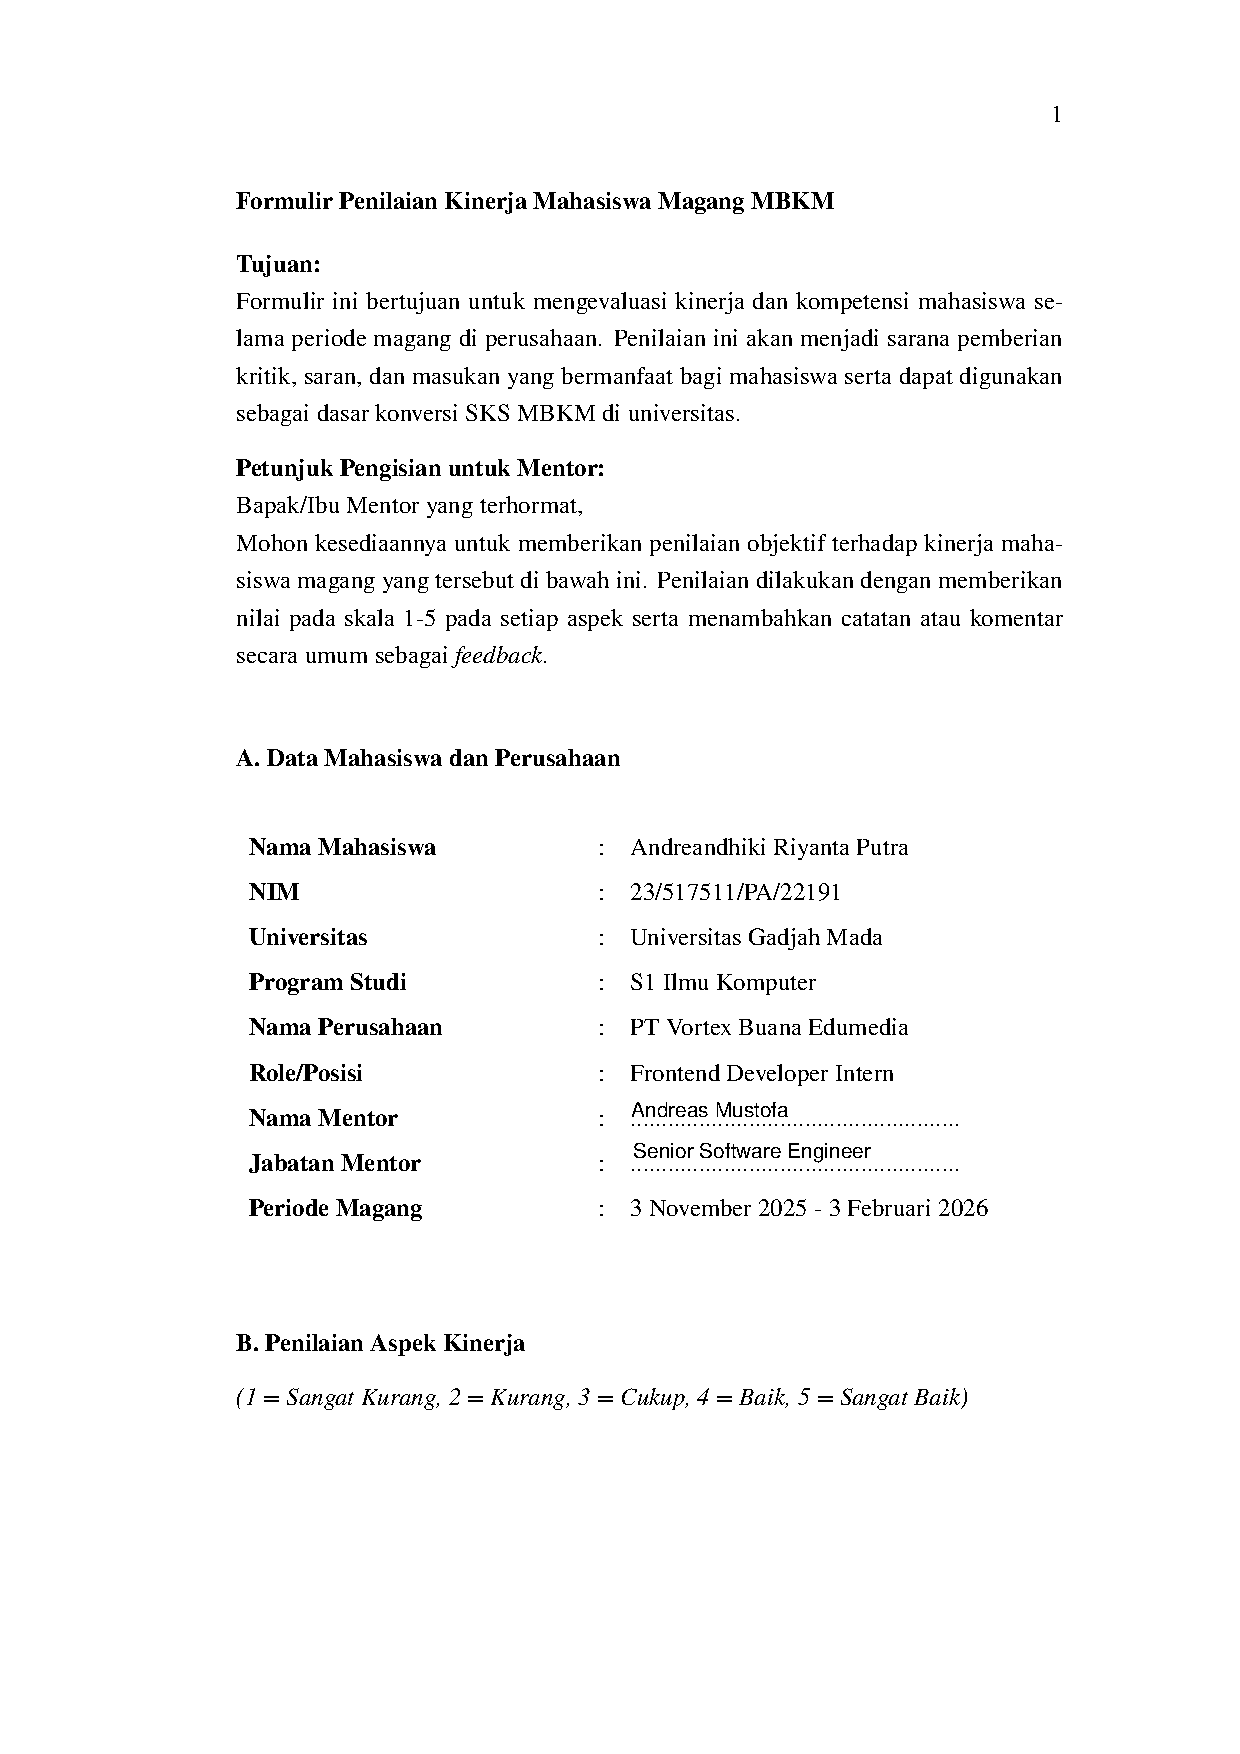
\includepdf[
	pages=-,
	frame=true,
	scale=0.8,
	pagecommand={\thispagestyle{fancy}}
]{assets/form_penilaian_mbkm_andreandhiki_riyanta_putra.pdf}


\chapter{Internship: Pengembangan Fitur dan Modul Proyek}

\section{Identitas Mata Kuliah}
\begingroup
\renewcommand{\arraystretch}{1.15}
\noindent\begin{tabular}{@{}p{3.6cm}@{\hspace{0.2cm}}p{0.2cm}@{\hspace{0.2cm}}p{7.6cm}@{}}
    \textbf{Kode Mata Kuliah} & : & MII21-3011 \\
    \textbf{Nama Mata Kuliah} & : & Internship: Pengembangan Fitur dan Modul Proyek \\
    \textbf{Bobot} & : & 4 SKS \\
    \textbf{Bentuk Kegiatan} & : & Magang MBKM sebagai Software Engineer Intern di OPPO Manufacturing Indonesia \\
    \textbf{Proyek Terkait} & : & 360 Peer-to-Peer Grading System dan PQPR Software Project \\
\end{tabular}
\par\vspace{0.5\baselineskip}
\endgroup

Mata kuliah ini berfokus pada penerapan kemampuan pengembangan fitur dan modul perangkat lunak dalam lingkungan kerja industri. Selama kegiatan magang, capaian mata kuliah diwujudkan melalui kontribusi pada dua proyek internal perusahaan, yaitu 360 Peer-to-Peer Grading System dan PQPR Software Project. Kedua proyek tersebut menuntut pemahaman kebutuhan pengguna, perancangan alur kerja aplikasi, implementasi fitur, integrasi data, serta penyesuaian modul agar dapat digunakan dalam proses bisnis perusahaan.

\section{Silabus}
Silabus mata kuliah mencakup pengembangan fitur perangkat lunak berdasarkan kebutuhan pengguna, perancangan modul aplikasi, implementasi antarmuka dan logika bisnis, integrasi dengan sumber data, serta dokumentasi hasil pengembangan. Dalam konteks magang, silabus tersebut diterapkan melalui pengembangan sistem evaluasi kinerja antarkaryawan pada proyek 360 Peer-to-Peer Grading System dan pengembangan modul pendukung optimasi perubahan lini produksi pada PQPR Software Project.

Kegiatan pengembangan fitur tidak hanya menekankan penulisan kode, tetapi juga kemampuan menerjemahkan kebutuhan bisnis menjadi rancangan teknis yang dapat diimplementasikan. Setiap fitur perlu memiliki tujuan yang jelas, alur penggunaan yang dapat dipahami, dan keluaran yang sesuai dengan kebutuhan operasional pengguna.

\section{Aktivitas}
Pada proyek 360 Peer-to-Peer Grading System, aktivitas pengembangan diarahkan pada penyusunan fitur yang mendukung proses penilaian rekan kerja secara terstruktur. Fitur yang dikembangkan mencakup alur pengisian penilaian, pengelolaan data evaluasi, tampilan rekapitulasi, serta mekanisme yang membantu pengguna menyelesaikan proses penilaian dengan konsisten. Pengembangan dilakukan dengan memperhatikan kemudahan penggunaan karena sistem ditujukan untuk pengguna dari berbagai tingkat jabatan dan latar belakang teknis.

Pada PQPR Software Project, aktivitas pengembangan berfokus pada modul yang membantu proses changeover produk di lingkungan manufaktur. Modul tersebut berkaitan dengan pengelolaan informasi produk, penyusunan konfigurasi lini produksi, serta pemanfaatan data kemampuan operator untuk mendukung keputusan operasional. Pengembangan fitur pada proyek ini membutuhkan pemahaman terhadap alur kerja pabrik, hubungan antar data produksi, dan kebutuhan pembaruan informasi secara akurat.

Selain implementasi fitur, aktivitas yang dilakukan juga meliputi diskusi kebutuhan dengan pembimbing dan anggota tim, pembacaan spesifikasi, penyesuaian rancangan berdasarkan umpan balik, serta perbaikan modul setelah dilakukan pengecekan. Aktivitas tersebut memperlihatkan bahwa pengembangan perangkat lunak di industri berlangsung secara iteratif dan membutuhkan koordinasi lintas peran.

\section{Konsep Dasar yang Berkaitan dengan Silabus}
Konsep utama yang digunakan dalam mata kuliah ini adalah pemecahan kebutuhan bisnis menjadi modul perangkat lunak yang memiliki tanggung jawab jelas. Modul yang baik perlu memiliki batas fungsi yang terdefinisi, masukan dan keluaran yang dapat dipahami, serta perilaku yang konsisten ketika digunakan bersama modul lain. Prinsip ini penting pada proyek 360 Peer-to-Peer Grading System karena alur penilaian, pengolahan data, dan penyajian hasil perlu saling terhubung tanpa menimbulkan kebingungan bagi pengguna.

Konsep lain yang digunakan adalah perancangan berbasis kebutuhan pengguna. Fitur tidak cukup hanya dapat berjalan secara teknis, tetapi harus sesuai dengan cara pengguna menyelesaikan pekerjaannya. Pada proyek PQPR Software Project, rancangan modul perlu mempertimbangkan konteks kerja manufaktur, seperti kebutuhan informasi yang cepat, data yang akurat, serta perubahan kondisi produksi yang dapat terjadi sewaktu-waktu.

Pengembangan fitur juga berkaitan dengan integrasi data dan validasi alur. Data yang dimasukkan, diproses, dan ditampilkan harus memiliki struktur yang konsisten agar modul dapat digunakan sebagai dasar pengambilan keputusan. Oleh karena itu, setiap rancangan fitur perlu memperhatikan relasi data, pembatasan akses, validasi masukan, dan kejelasan tampilan keluaran.

\section{Hasil dan Pembahasan}
Hasil utama dari pelaksanaan mata kuliah ini adalah meningkatnya kemampuan menerapkan proses pengembangan fitur secara utuh, mulai dari memahami kebutuhan hingga menghasilkan modul yang dapat digunakan dalam sistem internal perusahaan. Pada proyek 360 Peer-to-Peer Grading System, pengembangan fitur mendukung proses evaluasi kinerja yang lebih terstruktur dan terdokumentasi. Sistem membantu proses pengumpulan umpan balik sehingga data penilaian dapat dikelola dengan lebih rapi dibandingkan proses manual.

Pada PQPR Software Project, modul yang dikembangkan mendukung kebutuhan perusahaan dalam mengelola informasi produksi dan konfigurasi changeover. Dengan adanya modul yang terintegrasi, informasi produk dan kemampuan operator dapat digunakan untuk membantu penyusunan konfigurasi lini yang lebih efisien. Hal ini menunjukkan keterkaitan langsung antara pengembangan perangkat lunak dan peningkatan efektivitas proses operasional di lingkungan manufaktur.

Pembahasan dari kegiatan ini menunjukkan bahwa pengembangan fitur di industri memerlukan keseimbangan antara aspek teknis dan pemahaman domain. Keputusan teknis perlu mempertimbangkan dampaknya terhadap pengguna, pemeliharaan sistem, dan kesesuaian dengan proses bisnis. Umpan balik dari pembimbing dan anggota tim menjadi bagian penting karena membantu memastikan bahwa fitur yang dibuat tidak hanya selesai secara implementasi, tetapi juga relevan dengan kebutuhan perusahaan.

\section{Kesimpulan}
Mata kuliah Internship: Pengembangan Fitur dan Modul Proyek terlaksana melalui kontribusi pada pengembangan 360 Peer-to-Peer Grading System dan PQPR Software Project. Kegiatan tersebut memberikan pengalaman dalam menerjemahkan kebutuhan bisnis menjadi fitur perangkat lunak, merancang modul yang terstruktur, melakukan integrasi data, serta menyesuaikan hasil pengembangan berdasarkan umpan balik. Pengalaman ini memperkuat pemahaman bahwa keberhasilan pengembangan fitur tidak hanya ditentukan oleh kemampuan teknis, tetapi juga oleh ketepatan memahami kebutuhan pengguna dan konteks operasional sistem.

\chapter{Internship: Pengujian Unit dan Modul Proyek}

\section{Identitas Mata Kuliah}
\begingroup
\renewcommand{\arraystretch}{1.15}
\noindent\begin{tabular}{@{}p{3.6cm}@{\hspace{0.2cm}}p{0.2cm}@{\hspace{0.2cm}}p{7.6cm}@{}}
    \textbf{Kode Mata Kuliah} & : & MII21-3015 \\
    \textbf{Nama Mata Kuliah} & : & Internship: Pengujian Unit dan Modul Proyek \\
    \textbf{Bobot} & : & 3 SKS \\
    \textbf{Bentuk Kegiatan} & : & Magang MBKM sebagai Software Engineer Intern di OPPO Manufacturing Indonesia \\
    \textbf{Proyek Terkait} & : & 360 Peer-to-Peer Grading System dan PQPR Software Project \\
\end{tabular}
\par\vspace{0.5\baselineskip}
\endgroup

Mata kuliah ini berfokus pada kemampuan melakukan pengujian terhadap unit dan modul perangkat lunak agar sistem yang dikembangkan memiliki perilaku yang sesuai dengan kebutuhan. Dalam kegiatan magang, pengujian dilakukan pada fitur-fitur yang berkaitan dengan proses evaluasi karyawan pada 360 Peer-to-Peer Grading System dan modul pendukung changeover produksi pada PQPR Software Project.

\section{Silabus}
Silabus mata kuliah mencakup pemahaman tujuan pengujian perangkat lunak, penyusunan skenario uji, pemeriksaan unit dan modul, validasi masukan dan keluaran, pelacakan kesalahan, debugging, serta dokumentasi hasil pengujian. Pengujian dilakukan untuk memastikan setiap bagian sistem bekerja sesuai rancangan sebelum digunakan dalam alur kerja yang lebih besar.

Dalam konteks proyek magang, pengujian tidak hanya dilakukan untuk menemukan kesalahan teknis, tetapi juga untuk memastikan bahwa fitur dapat digunakan dengan aman dan konsisten oleh pengguna internal perusahaan. Hal ini penting karena kesalahan pada modul evaluasi maupun modul produksi dapat memengaruhi keakuratan data dan kelancaran proses operasional.

\section{Aktivitas}
Pada proyek 360 Peer-to-Peer Grading System, aktivitas pengujian dilakukan terhadap alur pengisian penilaian, validasi data evaluasi, penyimpanan hasil, serta tampilan rekapitulasi. Skenario uji disusun berdasarkan kemungkinan penggunaan sistem, seperti pengguna mengisi data secara lengkap, pengguna melewati isian wajib, dan sistem menampilkan kembali hasil penilaian. Pengujian tersebut membantu memastikan bahwa proses evaluasi dapat berjalan terstruktur dan tidak menghasilkan data yang tidak valid.

Pada PQPR Software Project, pengujian dilakukan terhadap modul yang berkaitan dengan informasi produk, konfigurasi lini produksi, dan data kemampuan operator. Aktivitas pengujian mencakup pemeriksaan kesesuaian keluaran modul terhadap data masukan, pengecekan perubahan data, serta validasi bahwa informasi yang ditampilkan tetap konsisten setelah dilakukan pembaruan. Karena proyek ini berhubungan dengan proses manufaktur, pengujian perlu memperhatikan akurasi data dan keterlacakan perubahan.

Aktivitas lain yang dilakukan adalah debugging terhadap perilaku sistem yang tidak sesuai, melakukan pengecekan ulang setelah perbaikan, dan mendiskusikan hasil temuan dengan pembimbing maupun anggota tim. Setiap temuan pengujian digunakan sebagai dasar untuk memperbaiki fitur atau menyesuaikan logika modul agar lebih sesuai dengan kebutuhan pengguna.

\section{Konsep Dasar yang Berkaitan dengan Silabus}
Konsep dasar yang digunakan dalam pengujian unit adalah memastikan bagian terkecil dari sistem bekerja sesuai tanggung jawabnya. Unit yang diuji perlu memiliki masukan yang jelas, keluaran yang dapat diprediksi, dan penanganan kondisi tidak valid. Konsep ini diterapkan pada validasi form, pengolahan data, dan fungsi pendukung yang digunakan dalam fitur penilaian maupun modul produksi.

Pengujian modul berfokus pada interaksi beberapa unit dalam satu alur kerja. Modul yang tampak benar secara terpisah masih dapat menghasilkan masalah ketika dihubungkan dengan modul lain. Oleh karena itu, pengujian modul perlu memperhatikan alur data, perubahan status, hubungan antar fitur, dan kesesuaian keluaran dengan kebutuhan bisnis.

Konsep lain yang berkaitan adalah debugging dan regresi. Debugging dilakukan untuk menemukan penyebab perilaku yang tidak sesuai, sedangkan pengecekan regresi dilakukan untuk memastikan perbaikan tidak merusak fungsi yang sebelumnya sudah berjalan. Dalam proyek magang, kedua konsep tersebut penting karena fitur dikembangkan secara bertahap dan mengalami penyesuaian berdasarkan umpan balik.

\section{Hasil dan Pembahasan}
Hasil dari pelaksanaan mata kuliah ini adalah meningkatnya kemampuan menyusun dan menjalankan pengujian yang relevan terhadap modul perangkat lunak. Pada 360 Peer-to-Peer Grading System, pengujian membantu memastikan bahwa alur evaluasi karyawan berjalan sesuai rancangan, data yang wajib diisi dapat divalidasi, dan hasil penilaian dapat ditampilkan dengan konsisten. Hal ini mendukung keandalan sistem sebagai sarana pengumpulan umpan balik internal.

Pada PQPR Software Project, pengujian membantu memastikan bahwa modul yang digunakan untuk mendukung proses changeover produksi menampilkan informasi yang tepat dan merespons perubahan data dengan benar. Validasi terhadap data produk dan kemampuan operator menjadi bagian penting karena informasi tersebut digunakan untuk mendukung keputusan operasional. Pengujian yang dilakukan membantu mengurangi risiko kesalahan data pada sistem.

Pembahasan kegiatan menunjukkan bahwa pengujian perangkat lunak perlu dilakukan sejak proses pengembangan berlangsung, bukan hanya pada akhir pengerjaan. Dengan pengujian bertahap, kesalahan dapat ditemukan lebih awal dan perbaikan dapat dilakukan sebelum masalah menyebar ke modul lain. Pengujian juga menjadi sarana komunikasi teknis karena hasil temuan perlu dijelaskan kepada anggota tim agar perbaikan dapat dilakukan secara tepat.

\section{Kesimpulan}
Mata kuliah Internship: Pengujian Unit dan Modul Proyek terlaksana melalui aktivitas penyusunan skenario uji, validasi fitur, debugging, dan pengecekan ulang pada 360 Peer-to-Peer Grading System serta PQPR Software Project. Kegiatan ini memperkuat pemahaman bahwa kualitas perangkat lunak bergantung pada kemampuan menguji perilaku sistem secara sistematis. Pengujian yang baik membantu memastikan modul bekerja sesuai kebutuhan, data tetap konsisten, dan sistem lebih siap digunakan dalam lingkungan kerja perusahaan.

\chapter{Soft Skill: Kemampuan Berkomunikasi}

\section{Identitas Mata Kuliah}
\begingroup
\renewcommand{\arraystretch}{1.15}
\noindent\begin{tabular}{@{}p{3.6cm}@{\hspace{0.2cm}}p{0.2cm}@{\hspace{0.2cm}}p{7.6cm}@{}}
    \textbf{Kode Mata Kuliah} & : & MII21-4010 \\
    \textbf{Nama Mata Kuliah} & : & Soft Skill: Kemampuan Berkomunikasi \\
    \textbf{Bobot} & : & 2 SKS \\
    \textbf{Bentuk Kegiatan} & : & Magang MBKM sebagai Software Engineer Intern di OPPO Manufacturing Indonesia \\
    \textbf{Proyek Terkait} & : & 360 Peer-to-Peer Grading System dan PQPR Software Project \\
\end{tabular}
\par\vspace{0.5\baselineskip}
\endgroup

Mata kuliah ini menekankan kemampuan berkomunikasi dalam lingkungan kerja profesional. Pada kegiatan magang, komunikasi menjadi bagian penting dalam memahami kebutuhan proyek, menyampaikan perkembangan pekerjaan, menjelaskan kendala teknis, menerima umpan balik, dan berkoordinasi dengan anggota tim yang memiliki peran berbeda.

\section{Silabus}
Silabus mata kuliah mencakup komunikasi lisan dan tertulis, penyampaian gagasan secara terstruktur, komunikasi dalam tim, kemampuan mendengarkan, pemberian dan penerimaan umpan balik, serta penyesuaian gaya komunikasi dengan lawan bicara. Dalam kegiatan magang, capaian tersebut diterapkan dalam interaksi dengan pembimbing lapangan, anggota tim teknis, pengguna internal, serta pihak yang memahami proses bisnis perusahaan.

Kemampuan komunikasi diperlukan karena pengembangan perangkat lunak tidak hanya dilakukan melalui aktivitas teknis. Setiap keputusan pengembangan perlu dijelaskan, setiap kebutuhan perlu dikonfirmasi, dan setiap perubahan perlu dikomunikasikan agar pekerjaan tim tetap selaras.

\section{Aktivitas}
Pada proyek 360 Peer-to-Peer Grading System, komunikasi dilakukan untuk memahami kebutuhan proses evaluasi karyawan dan memastikan alur sistem sesuai dengan tujuan pengguna. Diskusi dengan pembimbing dan anggota tim membantu memperjelas bentuk data yang perlu dikumpulkan, cara pengguna berinteraksi dengan sistem, serta informasi apa saja yang perlu ditampilkan dalam rekapitulasi penilaian.

Pada PQPR Software Project, komunikasi menjadi lebih penting karena proyek berkaitan dengan proses manufaktur yang memiliki istilah, aturan, dan kebutuhan operasional khusus. Penulis perlu memahami penjelasan dari pihak yang lebih mengetahui alur produksi, kemudian menerjemahkannya menjadi kebutuhan teknis yang dapat diterapkan dalam modul perangkat lunak. Proses ini membutuhkan kemampuan bertanya secara tepat, mencatat informasi penting, dan mengonfirmasi kembali pemahaman agar tidak terjadi kesalahan interpretasi.

Aktivitas komunikasi juga dilakukan melalui penyampaian progres pekerjaan, pelaporan kendala, diskusi perbaikan, dan penerimaan masukan terhadap fitur yang sedang dikembangkan. Dalam beberapa kondisi, kendala teknis perlu dijelaskan dengan bahasa yang mudah dipahami agar anggota tim nonteknis tetap dapat memahami dampaknya terhadap proses bisnis.

\section{Konsep Dasar yang Berkaitan dengan Silabus}
Konsep dasar yang digunakan adalah komunikasi dua arah. Komunikasi yang efektif tidak hanya berarti mampu menyampaikan pendapat, tetapi juga mampu mendengarkan, memahami konteks, dan memastikan pesan yang diterima sesuai dengan maksud pengirim. Konsep ini penting dalam kegiatan magang karena kebutuhan proyek sering kali berkembang setelah dilakukan diskusi dan evaluasi.

Konsep berikutnya adalah komunikasi lintas peran. Dalam proyek perangkat lunak, pengembang perlu berinteraksi dengan pembimbing, anggota tim teknis, pengguna, dan pihak operasional. Setiap pihak memiliki sudut pandang yang berbeda. Oleh karena itu, penyampaian informasi perlu disesuaikan dengan kebutuhan lawan bicara, misalnya menggunakan istilah teknis saat berdiskusi dengan tim pengembang dan menggunakan penjelasan proses saat berdiskusi dengan pengguna.

Kemampuan memberikan dan menerima umpan balik juga menjadi konsep penting. Umpan balik dari pembimbing dan pengguna membantu memperbaiki rancangan fitur, sedangkan kemampuan menyampaikan temuan atau usulan secara sopan dan terstruktur membantu proses pengambilan keputusan. Dengan komunikasi yang baik, perbaikan dapat dilakukan tanpa menghambat kerja sama tim.

\section{Hasil dan Pembahasan}
Hasil dari pelaksanaan mata kuliah ini adalah meningkatnya kemampuan berkomunikasi dalam konteks kerja profesional, terutama pada proyek perangkat lunak yang melibatkan kebutuhan teknis dan bisnis. Penulis belajar menyampaikan progres pekerjaan secara ringkas, menjelaskan kendala berdasarkan dampaknya terhadap pekerjaan, dan meminta klarifikasi ketika terdapat kebutuhan yang belum jelas.

Pada 360 Peer-to-Peer Grading System, komunikasi membantu memastikan bahwa fitur yang dikembangkan sesuai dengan kebutuhan proses evaluasi. Pada PQPR Software Project, komunikasi membantu menjembatani pemahaman antara kebutuhan operasional manufaktur dan implementasi teknis dalam sistem. Kedua pengalaman tersebut menunjukkan bahwa komunikasi berperan langsung terhadap ketepatan hasil pengembangan.

Pembahasan kegiatan menunjukkan bahwa kemampuan komunikasi menjadi faktor pendukung produktivitas tim. Kesalahan pemahaman dapat menyebabkan fitur tidak sesuai kebutuhan, sedangkan komunikasi yang jelas dapat mempercepat penyelesaian masalah. Dalam lingkungan magang, kemampuan untuk aktif bertanya, mencatat arahan, dan menindaklanjuti umpan balik menjadi kebiasaan kerja yang penting.

\section{Kesimpulan}
Mata kuliah Soft Skill: Kemampuan Berkomunikasi terlaksana melalui interaksi sehari-hari selama pengerjaan 360 Peer-to-Peer Grading System dan PQPR Software Project. Kegiatan ini memperkuat kemampuan menyampaikan ide, memahami kebutuhan pengguna, berdiskusi lintas peran, dan menerima umpan balik secara profesional. Kemampuan komunikasi terbukti menjadi bagian penting dari keberhasilan pengembangan perangkat lunak karena membantu memastikan pekerjaan teknis tetap sesuai dengan kebutuhan bisnis dan tujuan tim.

\chapter{Penutup}

\section{Kesimpulan}
Berdasarkan kegiatan MBKM di PT Vortex Buana Edumedia dan pembahasan pada bab-bab sebelumnya, dapat disimpulkan bahwa magang memberikan pengalaman langsung dalam pengembangan perangkat lunak pada lingkungan industri. Penulis berkontribusi pada pengembangan dokumentasi dan \textit{design library} Neon Interfaces serta fitur Import Nilai Neon Uji pada repositori Pendidikan. Kedua pekerjaan tersebut memiliki fokus berbeda, tetapi sama-sama menuntut ketelitian dalam memahami kebutuhan, merancang alur, mengembangkan fitur, menguji modul, dan berkomunikasi dengan tim.

Secara rinci, kesimpulan dari kegiatan ini adalah sebagai berikut:
\begin{enumerate}
    \item Mata kuliah Internship: Pengembangan Fitur dan Modul Proyek terlaksana melalui pengembangan dokumentasi komponen pada Neon Interfaces serta pengembangan fitur Import Nilai Neon Uji. Kegiatan tersebut memperkuat kemampuan menerjemahkan kebutuhan pengguna menjadi rancangan dan implementasi perangkat lunak yang relevan dengan kebutuhan perusahaan.
    \item Mata kuliah Internship: Pengujian Unit dan Modul Proyek terlaksana melalui penyusunan skenario uji, validasi fitur, debugging, dan pengecekan ulang pada modul yang dikembangkan. Pengujian membantu memastikan alur import nilai, pratinjau data, publikasi nilai, dan dokumentasi komponen memiliki perilaku yang konsisten.
    \item Mata kuliah Soft Skill: Kemampuan Berkomunikasi terlaksana melalui daily stand-up, diskusi design library, diskusi teknis fitur Import Nilai Neon Uji, training session intern, pelaporan progres, penyampaian kendala, dan penerimaan umpan balik. Kemampuan komunikasi terbukti penting untuk menjaga keselarasan antara pekerjaan teknis dan kebutuhan produk.
    \item Kegiatan magang memperlihatkan bahwa keberhasilan proyek perangkat lunak tidak hanya bergantung pada kemampuan implementasi, tetapi juga pada pemahaman domain, kualitas pengujian, dokumentasi yang baik, dan efektivitas komunikasi di dalam tim.
\end{enumerate}

Secara keseluruhan, kegiatan MBKM ini membantu menghubungkan pengetahuan akademik dengan praktik industri. Pengalaman tersebut menjadi bekal penting untuk memahami proses kerja profesional, standar kualitas perangkat lunak, dan tanggung jawab pengembang dalam menghasilkan sistem yang dapat digunakan oleh organisasi.

\section{Saran}
Saran yang dapat diberikan berdasarkan pelaksanaan kegiatan magang adalah sebagai berikut:
\begin{enumerate}
    \item Mahasiswa yang mengikuti kegiatan magang sebaiknya aktif mencatat kebutuhan, keputusan teknis, dan umpan balik selama proyek berlangsung agar proses pengembangan dan pengujian dapat ditelusuri dengan baik.
    \item Dalam pengembangan proyek perangkat lunak, pengujian sebaiknya dilakukan secara bertahap sejak awal implementasi. Cara ini membantu menemukan kesalahan lebih cepat dan mengurangi risiko perubahan yang merusak fitur lain.
    \item Dokumentasi komponen dan fitur sebaiknya dibuat seiring proses pengembangan. Dokumentasi yang baik membantu anggota tim lain memahami penggunaan komponen, alur fitur, dan batasan sistem.
    \item Komunikasi dengan pembimbing dan anggota tim perlu dilakukan secara rutin. Klarifikasi kebutuhan dan penyampaian progres yang jelas dapat membantu menjaga hasil pekerjaan tetap sesuai dengan tujuan proyek.
    \item Untuk pelaksanaan MBKM berikutnya, dokumentasi kegiatan dan keterkaitan dengan mata kuliah sebaiknya disusun sejak awal agar proses penyusunan laporan menjadi lebih terarah dan lengkap.
\end{enumerate}


% --- BAGIAN AKHIR ---
% Daftar Pustaka diaktifkan jika laporan sudah memiliki sitasi.
% \clearpage
% \addcontentsline{toc}{chapter}{Daftar Pustaka}
% \bibliographystyle{ieeetr}
% \bibliography{src/bibliography/references}

% --- LAMPIRAN ---
\clearpage
\appendix % Mengubah format BAB menjadi Lampiran A, B, dst.
% Mengubah penamaan bab menjadi "Lampiran A", "Lampiran B", dst otomatis oleh LaTeX
\chapter{Tautan Repositori dan Dokumentasi Antarmuka}

Berikut adalah beberapa tautan dokumentasi, rancangan antarmuka (UI/UX), serta repositori kode yang dikerjakan selama masa magang untuk pengembangan sistem *frontend*:

\section*{1. Rancangan UI/UX (Figma)}
Seluruh rancangan antarmuka pengguna, komponen *design system*, dan purwarupa interaktif dapat diakses melalui tautan berikut: \\
\url{https://www.figma.com/file/dummy-link-rancangan-sistem}

\section*{2. Repositori Source Code (GitHub / GitLab)}
Repositori utama yang berisi implementasi kode menggunakan React/Next.js beserta dokumentasi teknisnya dapat diakses pada: \\
\url{https://github.com/organisasi-dummy/frontend-project-repo}

\section*{3. Dokumentasi Tampilan Website (Live Demo)}
Sistem yang telah di-*deploy* ke *environment staging* untuk keperluan pengujian dapat diakses melalui: \\
\url{https://staging.dummy-project.com}

\vspace{1cm}

\chapter{Dokumentasi Kegiatan Lapangan}

\begin{figure}[htbp]
    \centering
    % Placeholder untuk foto kegiatan, ganti dengan \includegraphics[width=0.8\textwidth]{foto-kegiatan.jpg}
    \rule{12cm}{7cm}
    \caption{Tangkapan layar hasil implementasi komponen UI pada sprint ke-3}
    \label{fig:lampiran_kegiatan1}
\end{figure}

\begin{figure}[htbp]
    \centering
    \rule{12cm}{7cm}
    \caption{Diskusi penyesuaian integrasi API bersama tim *Backend*}
    \label{fig:lampiran_kegiatan2}
\end{figure}

\chapter{Lampiran LOA}

\section*{1. Letter of Acceptance}
\begin{figure}[htbp]
    \centering
    
\includegraphics[width=\textwidth,height=0.72\textheight,keepaspectratio,page=1]{assets/LOA.pdf}
    \caption{Letter of Acceptance (halaman pertama)}
    \label{fig:lampiran_loa}
\end{figure}

\end{document}
